\documentclass[11pt]{article}

\usepackage[margin=1in]{geometry}
\usepackage{amsmath, amssymb}
\usepackage{booktabs}
\usepackage{graphicx}
\usepackage{float}
\usepackage{hyperref}
\usepackage{natbib}
\usepackage{setspace}

\setlength{\parskip}{4pt}
\onehalfspacing

\title{\textbf{Three Preference Types in a Concave Public Goods Game}\\[4pt]
\large Equilibrium Strategies, Assortative Matching, and Replicator Dynamics}
\author{}
\date{}

\begin{document}

\maketitle

\noindent
This note studies the evolutionary selection among three discrete preference types---Homo Oeconomicus (H), Homo Kantiensis (K), and Pure Altruist (A)---in a two-player concave public goods game with assortative matching. The setup instantiates the homo moralis framework of \citet{AlgerWeibull2013} at the two polar Kantian weights ($\kappa = 0$ for H, $\kappa = 1$ for K) together with the pure altruistic benchmark.

%-----------------------------------------------------------------------
\section{Game}
%-----------------------------------------------------------------------

Player $i$'s material payoff when she contributes $x_i \in [0,1]$ and her opponent contributes $x_j$:
\begin{equation}
    \pi(x_i,\, x_j) \;=\; r(x_i + x_j) - \frac{r(x_i+x_j)^2}{2} - x_i, \qquad r = 3.
    \label{eq:pgg}
\end{equation}
The concave structure ($-r z^2/2$ congestion term) ensures all three types have distinct interior equilibrium strategies and separates their fitness profiles in a non-degenerate way.

%-----------------------------------------------------------------------
\section{Preference Types and First-Order Conditions}
%-----------------------------------------------------------------------

Each type maximises a utility function $u_i$ over own contribution $x$. Equilibrium strategies are derived by imposing the \textbf{within-type symmetry condition} $x = y$: each agent optimises under the assumption of facing an opponent of the \emph{same type} playing the \emph{same strategy}. Population composition $\{s_j\}$ is not observed by agents and does not enter the individual optimisation; it appears only in the fitness aggregation (Section~\ref{sec:fitness}).

\begin{table}[H]
    \centering
    \caption{Preference types, utility functions, and equilibrium strategies ($r=3$)}
    \label{tab:types}
    \begin{tabular}{lllll}
        \toprule
        Label & Type & Utility $u_i$ & $x_i^*$ (formula) & $x_i^*$ ($r=3$) \\
        \midrule
        H & Homo Oeconomicus & $\pi(x,\,y)$   & $\dfrac{r-1}{2r}$   & $0.333$ \\[8pt]
        K & Homo Kantiensis  & $\pi(x,\,x)$   & $\dfrac{2r-1}{4r}$  & $0.417$ \\[8pt]
        A & Pure Altruist    & $\pi(y,\,x)$   & $\dfrac{1}{2}$      & $0.500$ \\
        \bottomrule
    \end{tabular}
\end{table}

\paragraph{H: FOC.}
$u_H = r(x+y) - \tfrac{r(x+y)^2}{2} - x$.
\[
    \frac{\partial u_H}{\partial x} = r - r(x+y) - 1 = 0
    \;\xrightarrow{x=y}\;
    x_H^* = \frac{r-1}{2r}.
\]
The $-1$ term from the private cost $-x$ suppresses H's contribution below the social optimum.

\paragraph{K: FOC.}
$u_K = \pi(x,x) = 2rx - 2rx^2 - x$.
\[
    \frac{\partial u_K}{\partial x} = 2r - 4rx - 1 = 0
    \implies
    x_K^* = \frac{2r-1}{4r} \;=\; x_{\mathrm{soc}}^*.
\]
K's equilibrium coincides exactly with the social optimum (the contribution that maximises aggregate welfare $2\pi(x,x)$).

\paragraph{A: FOC.}
$u_A = \pi(y,x) = r(y+x) - \tfrac{r(y+x)^2}{2} - y$. The cost term $-y$ (opponent's cost) vanishes under $\partial/\partial x$:
\[
    \frac{\partial u_A}{\partial x} = r - r(y+x) = 0
    \;\xrightarrow{x=y}\;
    x_A^* = \frac{1}{2}.
\]
No private-cost brake: A over-contributes beyond the social optimum.

\paragraph{Ordering.} For all $r > 1$:
\[
    x_H^* \;=\; \frac{r-1}{2r} \;<\; x_K^* \;=\; \frac{2r-1}{4r} \;=\; x_{\mathrm{soc}}^* \;<\; x_A^* \;=\; \frac{1}{2}.
\]

%-----------------------------------------------------------------------
\section{Assortative Matching, Fitness, and Replicator Dynamics}
\label{sec:fitness}
%-----------------------------------------------------------------------

\paragraph{Assortativity.} Each agent meets a like-type partner with probability $\sigma \in [0,1]$ and a random draw from the current population with probability $1-\sigma$.

\paragraph{Fitness.} Expected material payoff of type $i$:
\begin{equation}
    f_i \;=\; \sigma\,\pi(x_i^*,\, x_i^*) \;+\; (1-\sigma)\sum_j s_j\,\pi(x_i^*,\, x_j^*),
    \label{eq:fitness}
\end{equation}
where $s_j$ is type $j$'s current population share. Fitness measures \emph{material} payoff $\pi$, not utility---evolution selects on outcomes, not intentions.

\paragraph{Replicator equation.}
\begin{equation}
    s_i(t+1) \;=\; s_i(t) \;+\; s_i(t)\,\bigl(f_i(t) - \bar{f}(t)\bigr),
    \qquad \bar{f}(t) = \sum_j s_j(t)\,f_j(t).
    \label{eq:replicator}
\end{equation}
Types with above-average fitness expand; those with below-average fitness contract; shares sum to one.

%-----------------------------------------------------------------------
\section{Simulation Results}
%-----------------------------------------------------------------------

\noindent\textbf{Parameters:} $r=3$, $N = 800$ generations, initial equal shares $s_H = s_K = s_A = 1/3$, $\sigma \in \{0.0,\,0.25,\,0.40,\,0.80\}$.

\begin{table}[H]
    \centering
    \caption{Steady-state population shares}
    \label{tab:results}
    \begin{tabular}{lrrrl}
        \toprule
        $\sigma$ & $s_H^*$ & $s_K^*$ & $s_A^*$ & Outcome \\
        \midrule
        0.00 & 1.000 & 0.000 & 0 & H dominates \\
        0.25 & 0.807 & 0.193 & 0 & H dominates, K coexists \\
        0.40 & 0.214 & 0.786 & 0 & interior equilibrium (K majority) \\
        0.80 & 0.000 & 1.000 & 0 & K dominates \\
        \bottomrule
    \end{tabular}
\end{table}

\noindent
The Pure Altruist is eliminated at all $\sigma$. This follows from a uniform dominance result: $\pi(x_A^*,\, x_j^*) < \pi(x_K^*,\, x_j^*)$ for every opponent type $j$, because A's over-contribution ($x_A^* > x_{\mathrm{soc}}^*$) yields lower material payoff than K's social-optimal contribution against any fixed opponent. A's self-inflicted efficiency loss is not offset by benefit to the partner in a game with diminishing returns.

\begin{figure}[H]
    \centering
    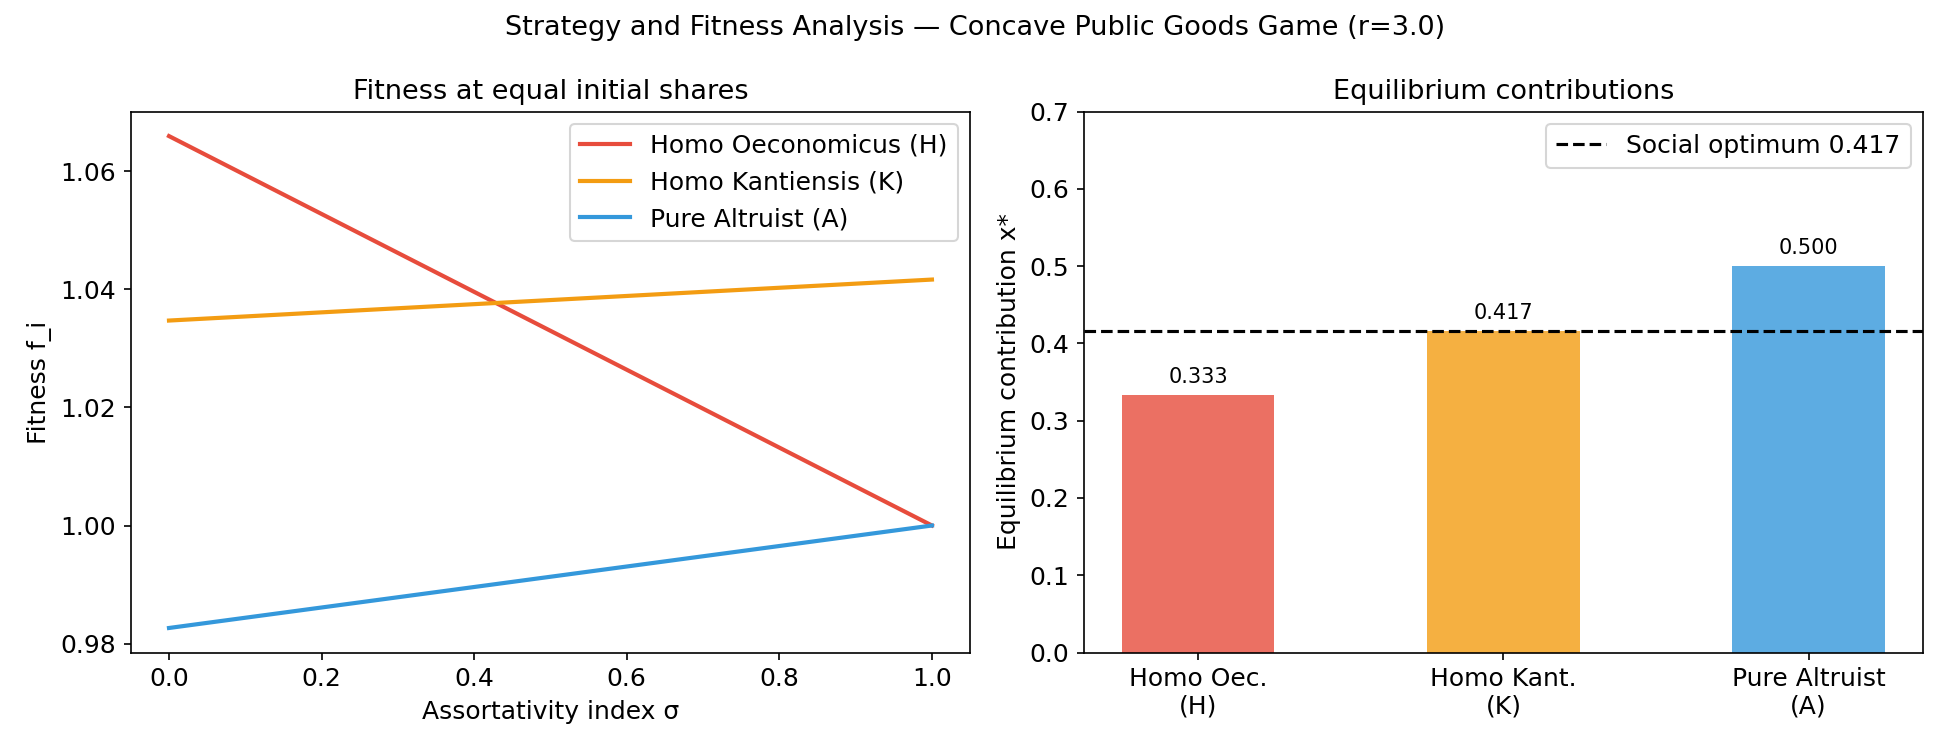
\includegraphics[width=\textwidth]{Code/pgg_fitness.png}
    \caption{Left: fitness of each type at equal initial shares as $\sigma$ varies. H fitness is highest at $\sigma=0$ and decreasing; K fitness is lowest at $\sigma=0$ and increasing; A is strictly dominated by K at every $\sigma$. Right: equilibrium contributions; dashed line = social optimum.}
    \label{fig:fitness}
\end{figure}

\begin{figure}[H]
    \centering
    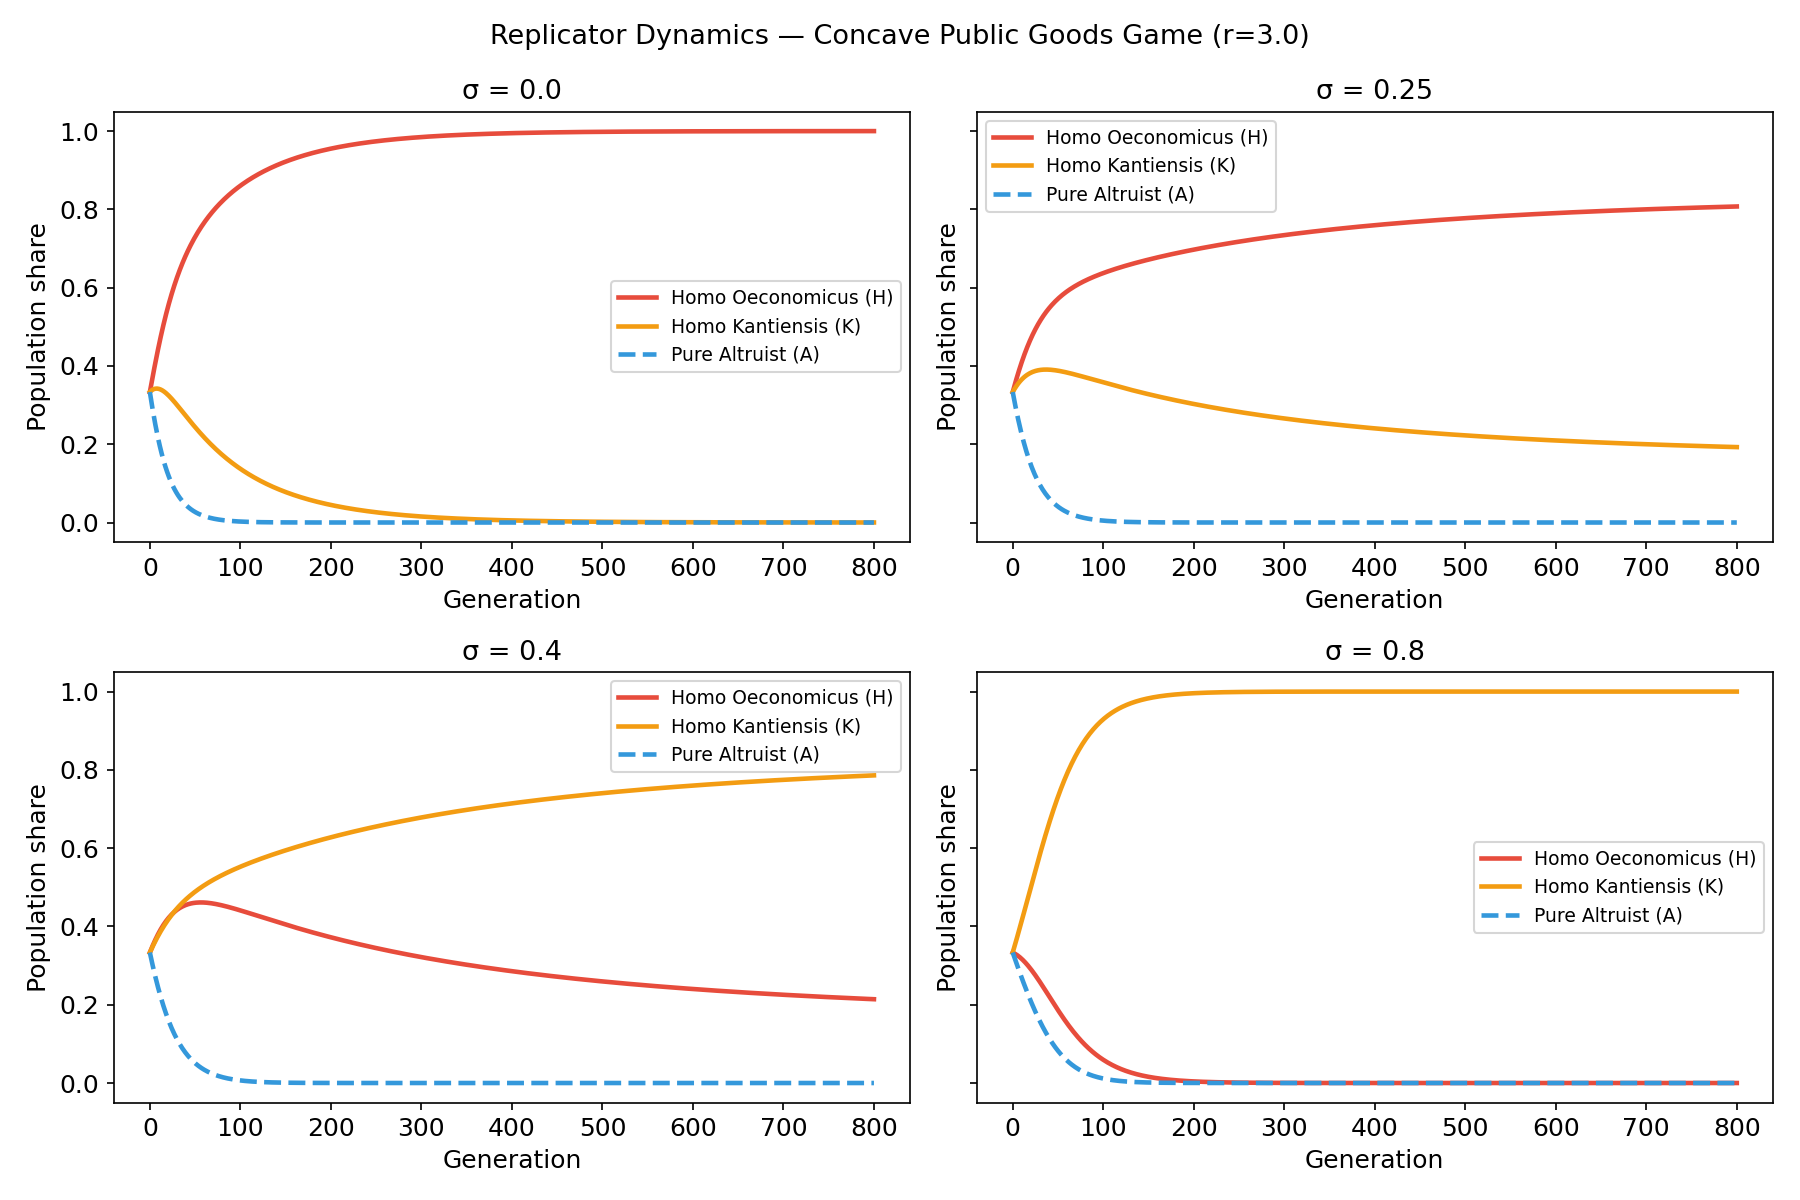
\includegraphics[width=\textwidth]{Code/pgg_population.png}
    \caption{Share trajectories over 800 generations. Note the transient at $\sigma=0.40$: H holds an early advantage in the mixed population before K accumulates sufficient critical mass to overtake.}
    \label{fig:population}
\end{figure}

\begin{figure}[H]
    \centering
    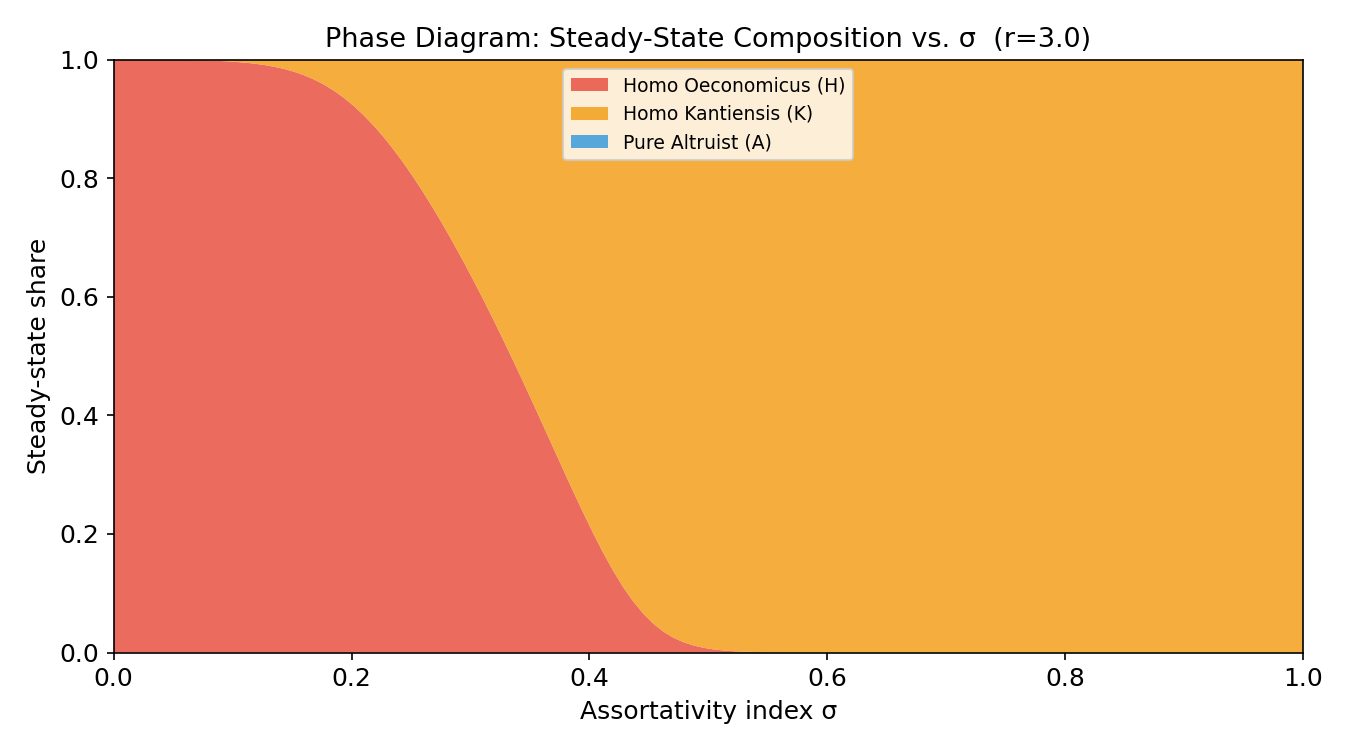
\includegraphics[width=0.85\textwidth]{Code/pgg_phase.png}
    \caption{Steady-state composition as a continuous function of $\sigma$. Phase transition at $\sigma \approx 0.35$; transition is S-shaped (slowest near critical point where fitness differentials are smallest). A share is zero throughout.}
    \label{fig:phase}
\end{figure}

\begin{figure}[H]
    \centering
    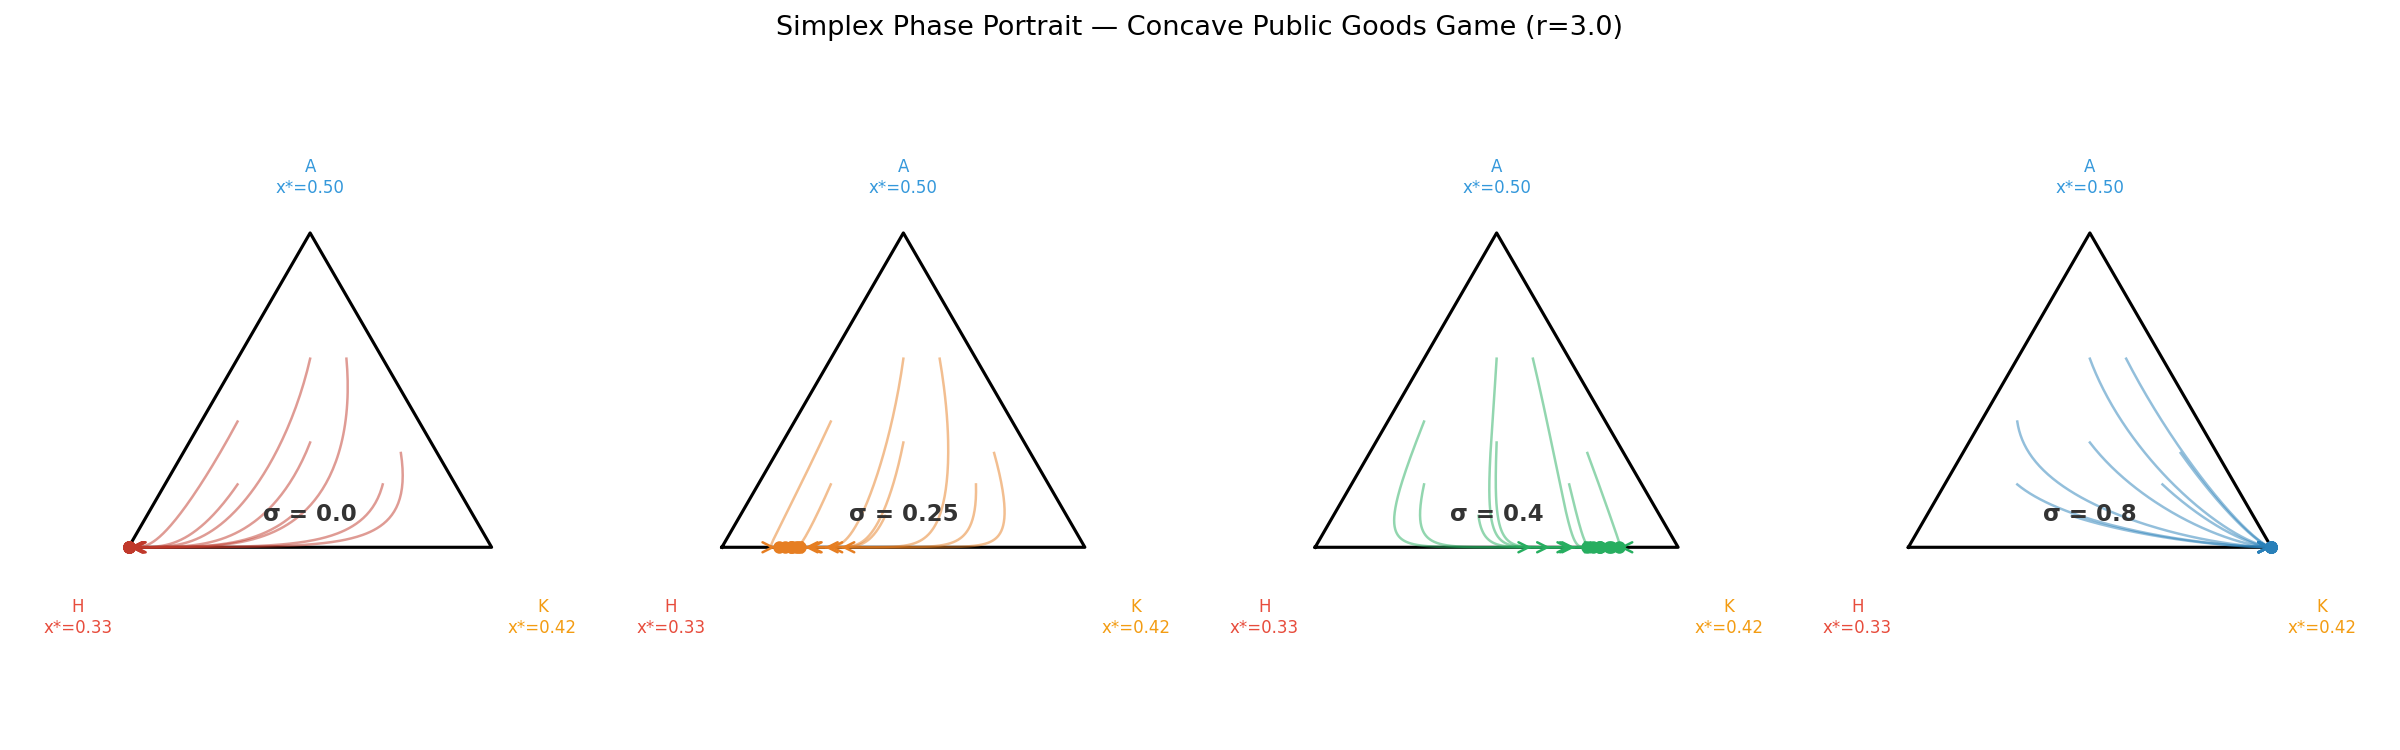
\includegraphics[width=\textwidth]{Code/pgg_simplex.png}
    \caption{Simplex phase portrait from eight initial conditions at each $\sigma$. The A vertex is never an attractor under any matching regime. At $\sigma=0.40$, several trajectories exhibit a detour toward H before reversing toward the K-majority interior equilibrium.}
    \label{fig:simplex}
\end{figure}

\paragraph{Key observation.}
The result is symmetric: in a concave game, evolution eliminates \emph{both} the under-contributor (H, at high $\sigma$) and the over-contributor (A, at all $\sigma$). The stable type is the one whose equilibrium contribution exactly coincides with the social optimum---Homo Kantiensis---whenever the social structure provides sufficient within-type interaction.

\bibliographystyle{plainnat}
\bibliography{references}

\end{document}
